\documentclass[]{cv-style} % Add 'print' in [] to get print-view
\usepackage{graphicx}
\usepackage{xeCJK}
\usepackage{setspace}
\begin{document}
\header{ }{  }
\begin{aside}
\section{.}
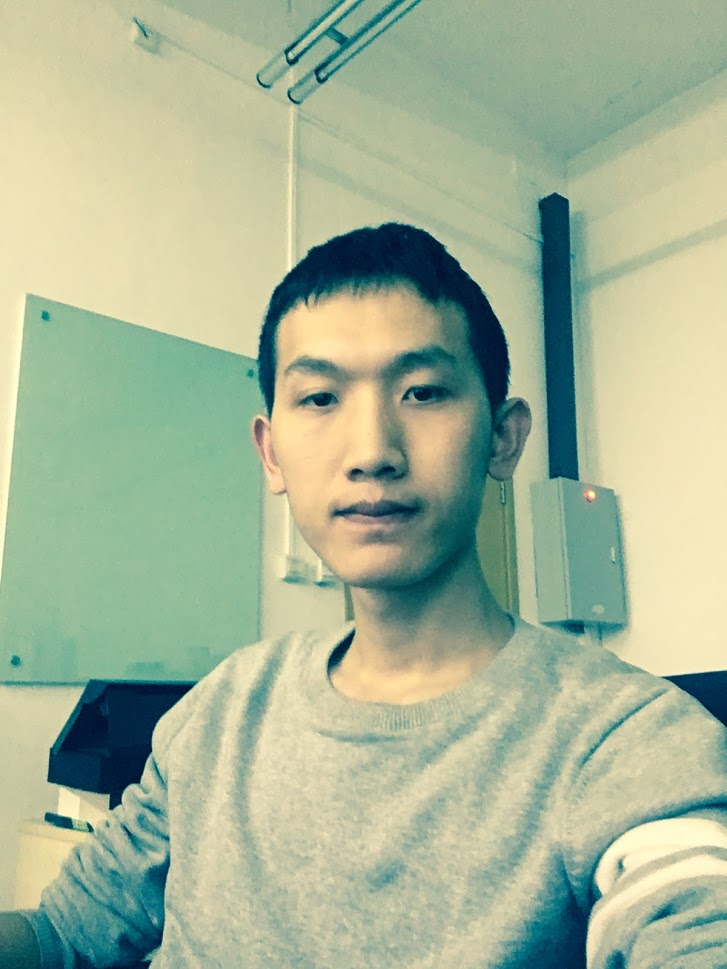
\includegraphics[width=4cm]{mathen}
\section{Contact}
网易游戏(杭州)
~
13581724604
~
hitminxuanwang\\@gmail.com
\section{Languages}
C++
Python
\section{Skills}
图形渲染OpenGL DX
图像处理OpenCV
\end{aside}
\section{Career Objective}
  \vspace{-0.2cm}
  \hspace{0.2cm}图形图像相关工作岗位,与图形图像相关的计算机视觉方向岗位,算法相关职位。
\section{Experience}
\begin{entrylist}

\entry
  {2018.7-Now}
  {图形学工程师}
  {网易游戏}
  {
    \vspace{-5pt}
    \leftmargini=-1cm
    \begin{itemize}
      \setlength{\itemsep}{3pt}
      \item {MINI项目, 负责一款卡通风格的客户端开发,使用Instancing构建场景,涉及\\水,草树木,
      雾效等,并进行移动端优化}
      \item {实时软阴影,水彩渲染论文实现,和美术合作开发各种游戏效果,负责游戏中\\的shader编写,同时参与了一些客户端的
      开发,并负责游戏的移动端优化}
    \end{itemize}
    \vspace{5pt}
    \hspace{-1.2cm} \textbf{keywords:} \emph{Rendering}, GPU Instancing, Shader,移动端优化, Unity, HLSL, Python
  }

\entry
  {2017.11-18.1}
  {实习生}
  {旷世科技}
  {
    \vspace{-5pt}
    \leftmargini=-1cm
    \begin{itemize}
      \setlength{\itemsep}{3pt}
      \item {提取人脸特征并快速检测Haar-like特征+积分图机制+级联分类器}
      \item {调研ImageCaption相关研究}
    \end{itemize}
    \vspace{5pt}
    \hspace{-1.2cm} \textbf{keywords:} \emph{Facial recognition, C++, LSTM}
  }

\entry
  {2017.6-7}
  {实习生}
  {网易游戏}
  {
    \vspace{-5pt}
    \leftmargini=-1cm
    \begin{itemize}
      \setlength{\itemsep}{3pt}
      \item {区别于传统计算方式,直接使用GPU生成光照贴图数据, 主要参考Unreal中的\\CPU的保守光栅, 移植到GPU端}
      \item {设置图像质量衡量指标筛选质量不达标的贴图}
    \end{itemize}
    \vspace{5pt}
    \hspace{-1.2cm} \textbf{keywords:} OpenGL, OpenCV, 图像处理, C++, Python
  }

\entry
  {2016 - 2017}
  {学生}
  {清华大学}
  {
    \vspace{-5pt}
    \leftmargini=-1cm
    \begin{itemize}
      \setlength{\itemsep}{3pt}
      \item {改进摄影构图的论文,根据用户拍摄的图像进行合适的构图推荐}
      \item {应用APAP算法完成多图像对齐}
      \item {实现比较多种图像融合算法:Multi-Splines,Modified Poission,Convolution\\ Pyramid
      , Multi-Band,Mean-Value Coordinates等}
      \item {使用RealismCNN训练分类网络来检测融合结果中的色彩渗透现象}
      \item {提出改进的卷积金字塔方法消除色彩渗透,生成效果更好的全景视频}
    \end{itemize}
    \vspace{5pt}
    \hspace{-1.2cm} \textbf{keywords:} \textbf{网格变换, 全景图像, 泊松方程, 调和插值, 频域卷积, 光照分离, 双向差值,}\\ {C++ , Caffe, CNN}
}

\end{entrylist}
\vspace{-10pt}
\section{Education}
\begin{entrylist}
\vspace{-10pt}
\entry
{2015 - 2018}
{图形学与计算几何实验室 {\normalfont ~~ 计算机专业~~清华大学}}
{ 硕士}
{}
\vspace{-10pt}
\entry
{2010 - 2014}
{计算机专业 {\normalfont ~~ 哈尔滨工业大学}}
{ 学士}
{ }
\end{entrylist}
\vspace{-5pt} 
\section{Publications}
\begin{entrylist}
\entry
{2018}
{A Comparative Study of Algorithms for Realtime Panoramic Video Blending.}
{TIP}
{ IEEE Trans. Image Processing 27(6): 2952-2965 (2018)}
\entry
{2017}
{Avoiding bleeding in image blending.}
{ICIP}
{IEEE International Conference on Image Processing}
\end{entrylist}
\vspace{-10pt}
\section{Awards}
\begin{entrylist}
  \vspace{5pt}
   \hspace{0.2cm}研究生期间的全景视频生成项目获得清华-腾讯联合实验室优秀项目奖\\
   \hspace{0.2cm}全景视频生成项目作为实验室项目的一部分参与了国家科技进步二等奖的申报并获奖
\end{entrylist}

\end{document}